\documentclass{article}
\usepackage[utf8]{inputenc}
\usepackage{graphicx}

\title{IE 498 HW2}
\author{Yifan Shi(yifans16)}
\date{February 20, 2020}

\begin{document}

\maketitle

I defined my filter of convolution to be 5x5 
with 32 channels. Since the input layer 
was 28x28 and I did not apply padding, the 
size of the hidden layer should be 24x24. 
The size of output layer was the same as the 
fully connected neural network which was 10x1. 
I initialized the kernel and the weight the 
same way as the weights in FCNN while the size 
of kernel was 32x$5^2$(for the vectorized 
operation) and the size of weight was 10x32x12x12. 
Bias was initialized as all zeros and learning rate 
$\alpha$ was 0.01


Then I wrote my own functions for transformation 
of the input layer, for mean pooling layer and 
for backward step of mean pooling. However, I 
used three pairs of nested for loops and I wonder 
if these could be replaced with vectorized 
operation. I also wanted to use the max pooling,
but I was not able to figure out how to put these 
max elements back to their original positions in 
the backward procedure. 


I did not use mini batch in my convolution network. So 
the input layer in each epoch was a single observation 
randomly chosen from $trn_x$. Then I reshaped my input as 
a square matrix and applied my tranformation function on 
it. Next I just multipled it with kernel and, reshaped the 
product back into 32x24x24 and applied the mean pooling 
function on it. Here I was also not sure if I should add 
the pooling layer at this step, or on the result from the 
activation function. The following steps were similar to 
FCNN until I applied the backward pooling on the dot 
product of $\sigma'(z)$ and $\delta$. 


I did all the operations for 3d and 4d arrays with the 
numpy.einsum(). I set the number of epoch to be 20000 
and I got 95 percent of prediction accuracy on the testing 
set. I also tried to adjust my parameters but the accuracy 
only dropped a little bit as a result. The best prediction 
accuracy on both training and tesing sets are shown below 
in Figure 1. 

\begin{figure}[h]
    \centering
    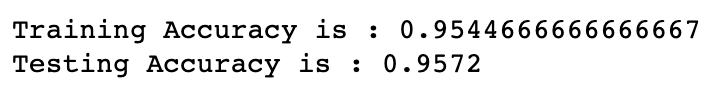
\includegraphics[scale=0.6]{accuracy.png}
  \end{figure}
\centering Figure\ 1: Prediction Accuracy.


\end{document}